% 版权声明 关于本书

\chapter*{版权声明}

小时物理百科是一个免费项目,项目网站为 \link{littleshi.cn}{http://littleshi.cn},网站免费提供本书的网页版和 pdf 版的下载更新.

为了维持项目不断发展,强烈建议每位读者试读超过 1 小时后在网站上捐款.我们在此表示衷心感谢.

若以任何方式转载本项目内容(包括插图,代码,网页等)需经过作者同意.

\chapter*{小时物理百科}

\subsection{简介}

小时物理百科(以下简称百科)从结构上尝试将教材和百科这两种不同形式的文本融合到一起,使其既适合初学者自学,又可按照非常灵活的顺序阅读.百科计划涵盖本科物理中的大部分内容,适用于具有普通高中及以上数学物理水平的读者\footnote{但也会适当复习部分高中内容.}.

百科是一个庞大的工程,短时间内很难被完成,所以百科将长期处于更新状态.为保证阅读质量,请定期从项目网站下载最新版.

在介绍百科的特点以前,我们先来看一般数理教材的不足:
\begin{enumerate}
\item 需要按顺序学习,不适合初学者快速了解或查找某个话题或知识点.例如某高中生需要了解角动量的概念,直接翻开力学书的相关章节发现看不懂,却又不知道需要先学什么,也没时间从头看教材.
\item 读者不能自己掌握所学内容的深度和严谨性.例如许多高等数学教材在读者对微积分还没有一个大概的了解时就介绍极限的 $\varepsilon-\delta$ 定义,微分/积分中值定理,可微,可积等.这些内容对物理的初步学习来说显得过于严谨.
\item 不够自洽(self-contained).一本教材的自洽性指目标读者在学习前是否还需要学习其他教材.大部分本科物理教材对高中生都是不自洽的,因为它们往往假设读者具有一定的微积分和线性代数基础.
\end{enumerate}

再来看一般网络百科(如百度百科或维基百科)的不足:
\begin{enumerate}
\item 每个词条都大而全,涵盖词条标题的所有相关内容.
\item 读者同样不能自己掌握所学内容的深度和严谨程度.
\item 容易出现公式定理的堆积,缺乏知识点导入和讲述,缺乏例题,习题等.
\end{enumerate}

\begin{figure}[ht]
\centering
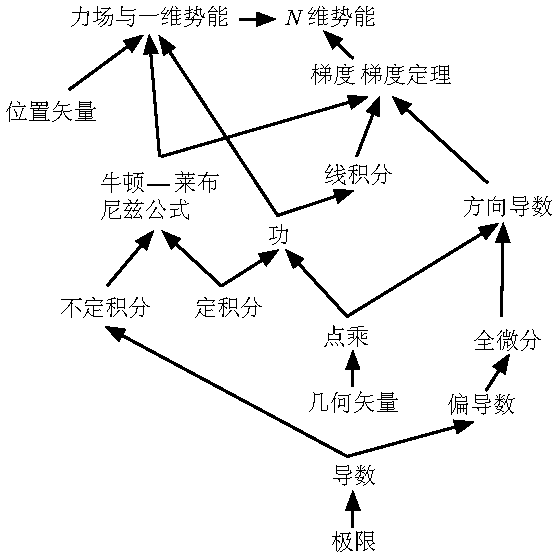
\includegraphics[width=10cm]{./figures/flowchart_example.pdf}
\caption{由“预备知识”画出的知识结构图(目标词条为“力场\ 势能\upref{V}”)}\label{FrontMatters_fig1}
\end{figure}

为了克服上述困难,百科采用以下形式:
\begin{enumerate}
\item 将知识点划分为词条,且在每个词条中列出学习该词条前需要先学习哪些词条.这样相当于建立了一个知识树(如\autoref{FrontMatters_fig1}).
\item 采用词条分级,把同一个话题以不同深度,严谨度和适用范围等划分成若干个等级的同名词条.这样读者可以选择螺旋式学习(例如初中,高中,大学物理中所学的话题几乎相同,但程度不同).暂定初级词条从科普开始,尽量少使用数学.随着词条级别升高,会使用适用范围更广的定义,更严谨的表述和更抽象的数学等.
\end{enumerate}

\subsection{词条}
百科内容繁多,不同词条的重要性相去甚远,不建议初学者按照词条的排列顺序依次学习,而是应该以初级词条给出的主线来学习,再根据兴趣和需要阅读其余词条.

理论上来说,读者可以直接跳到最感兴的词条,如果“预备知识”中列出的词条都已经掌握,就可以开始学习该词条,否则就先掌握“预备知识”中的词条.如果“预备知识”出现在词条开始,则必须先掌握,如果出现在正文中,则只有阅读该部分时需要掌握.如果正文中引用了没有出现在“预备知识”中的内容,则读者可自行决定是否阅读.

为了便于书内的跳查,词条之间进行了大量的交叉引用,例如“导数简介\upref{Der}” 右上角中括号中的数字代表被引用词条的页码. 由于每个词条的公式编号都从 1 开始, 引用其他词条中的公式有时会用类似“\autoref{Der_eq2}\upref{Der}” 的格式, 右上角的方括号中是公式所在词条的起始页码. 在本书的 PDF 电子版中,点击该页码即可自动跳转到对应的页面.在电脑上阅读,推荐使用 Adobe Reader 阅读器,在苹果\textsuperscript{\textregistered} 的 iOS 设备上推荐使用 GoodReader 应用( 两个软件都可以在不同的面板中打开同一本书的不同页码). 在 Adobe Reader 中,使用快捷键组合 “Alt +左箭头” 即可返回跳查前的位置,在移动设备的阅读软件中通常也有相应的返回按钮. 由于本书的电子版是原生 PDF(区别于扫描版), 还具有占用设备存储空间小, 便于分享, 便于查找关键字等种种优势.

%\subsection{5.本书符号约定}
%本书尽量使用物理学教科书中最常使用的符号,列出如下
%用粗体表示矢量,如 $\bvec F = m \bvec a$,用非粗体表示标量或矢量的模长,如 $\abs{\bvec F} = F$.同样用粗体表示矩阵,粗体上方加“$\^$”表示算符
% 未完成


% 物理学专业介绍 % 特别强调理科和工科的区别,介绍物理本科物理一般的学习内容
% 只学习最基础的规律,和模型,知识面广,但不复杂
% 由于太基础,会被认为“没有用”,离应用较远.
% 但物理又是其他理工科的基础
% 物理美在哪里? 更像是“艺术”,从几个最基本的假设出发,由数学推导出许多重要的结果.
% 本书遵循的理念:用尽可能少的公理,和尽可能简单的数学推导出结果,但有尽量保持严谨.
% 数学部分不可能做到像高等数学教材一样严谨,只求易懂且满足本书物理部分的使用.
% 均为本科物理专业教科书的标准内容,自己的内容或者超纲内容会在 “超纲内容” 部分中给出
